\begin{center}
    \begin{figure}[h]
      \centering
      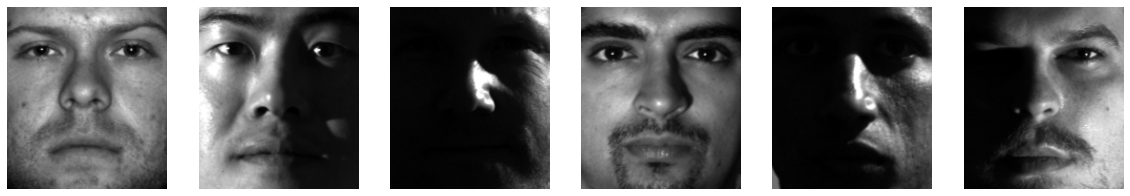
\includegraphics[width=0.86\linewidth]{external_content/media/eigenfaces.png}
      \captionsetup{justification=centering}
      \caption{Samples from the Eigenfaces data set \cite{georghiades2001few}}
      \label{fig:eigenfaces}
    \end{figure}
\end{center}
\vspace{-8mm}


\begin{minipage}[h][120mm][t]{0.35\linewidth}
    \begin{center}
        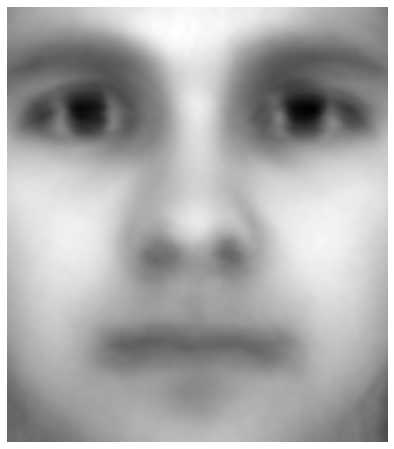
\includegraphics[width=0.81\linewidth]{external_content/media/eigenfaces/average_face.png}
        \captionsetup{justification=centering,type=htypei}
        \captionof{figure}{Average face}
        \label{fig:eigenfaceAVG}
    \end{center}
    \begin{center}
        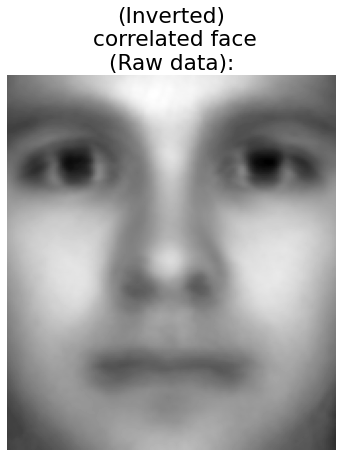
\includegraphics[width=0.81\linewidth]{external_content/media/eigenfaces/correlated_face-uncentered.png}
        \captionsetup{justification=centering,type=htypei}
        \captionof{figure}{Correlated face\\on uncentered data}
        \label{fig:eigenfaceCORRuncentered}
    \end{center}
    \begin{center}
        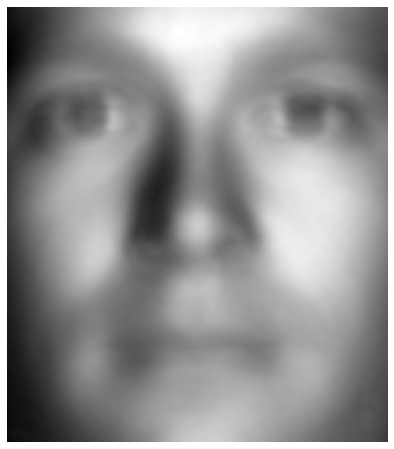
\includegraphics[width=0.81\linewidth]{external_content/media/eigenfaces/correlated_face-centered.png}
        \captionsetup{justification=centering,type=htypei}
        \captionof{figure}{Correlated face\\on centred data}
        \label{fig:eigenfaceCORR}
    \end{center}
\end{minipage}\hfill%
\begin{minipage}[h][120mm][t]{0.55\linewidth}

    % reset indentation
    \setlength{\parindent}{2em}

    \bigskip

    \noindent
    For this demonstration, we will introduce the Yale Face Database.
    The data set contains 2282 faces from 36 people under different lighting conditions.
    A few samples are depicted in figure \ref{fig:eigenfaces}.
    This data set will be the basis for the examples in the upcoming sections.

    \bigskip

    In figure \ref{fig:eigenfaceAVG} we see what the average of all faces looks like.
    We can observe blurriness transitions in selected areas where differences in facial traits are most distinctive such as the contours of the face or the edge of the nose.

    \medskip

    Meanwhile, the was taken from computing the correlation matrix on uncentered data in figure \ref{fig:eigenfaceCORRuncentered} looks nearly identical to the average face in figure \ref{fig:eigenfaceAVG}.
    The key difference is that the transitions areas appear darker instead of blurred.

    \medskip

    On the other hand, the correlated face on the centred data in figure \ref{fig:eigenfaceCORR} illustrates the data from a new perspective.
    We can observe that centring the data has given new opportunities, whether these are for better or for worse remains to be determined according to the circumstances of a given problem.

    % \item Difference centered and non-centered data
    % \item average face

\end{minipage}%
